\chapter{Godkendelsesformular}

{\LARGE\textit{Godkendelsesformular}}

Antal sider:  \pageref{LastPage}

\begin{figure}[H]
	\centering
	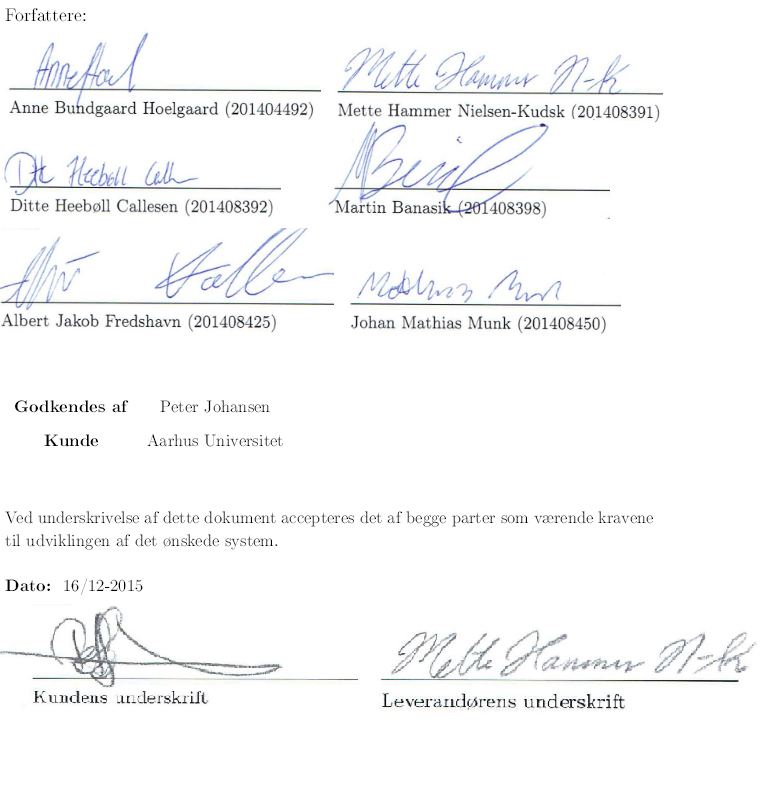
\includegraphics[width=1.\textwidth]{Figurer/godkendelsesformular}
	%\caption{SQL-kode til oprettelse af tabeller i database}
	%\label{fig:SQL-kode til oprettelse af tabeller i lokal database}
\end{figure}


%{\large Forfattere:}
%\\[5ex]


%\begin{tabular}{c c}
%\centering 
%	\makebox[2.0in]{\hrulefill} & \makebox[2.0in]{\hrulefill}\\
%	Anne Bundgaard Hoelgaard & Mette Hammer Nielsen-Kudsk\\[7ex]
%	\makebox[2.0in]{\hrulefill} & \makebox[2.0in]{\hrulefill}\\
%	Ditte Heebøll Callesen & Martin Banasik\\[7ex]
%	\makebox[2.0in]{\hrulefill} & \makebox[2.0in]{\hrulefill}\\
%	Albert Jakob Fredshavn & Johan Mathias Munk\\[7ex]
	

%\end{tabular}

%\begin{tabular}{c c c c}
%	\textbf{Godkendes af} & Peter Johansen\\[3ex]
%	\textbf{Antal sider} & \pageref{LastPage} \\[3ex]
%	\textbf{Kunde} & Aarhus Universitet
%\end{tabular}\\[8ex]
%Ved underskrivelse af dette dokument accepteres det af begge parter som værende kravene til udviklingen af det ønskede system.
%\\
%\\
%\textbf{Dato: } 16/12-2015\\[7ex]

%\begin{tabular}{c c}
%	\makebox[2.0in]{\hrulefill} & \makebox[2.0in]{\hrulefill}\\
%	\centering 
%	Kundens underskrift & Leverandørens underskrift
%\end{tabular}
